% !TEX root = main.tex
% ============================================================
% Fichier : modele_cinetique.tex
% EN COURS, partie à retravailler (Marcus, MHC à venir)
% ============================================================

\section*{Modèle cinétique}

La cinétique interfaciale relie la densité de courant $j$ à la surtension
locale $\eta = \varphi_s - \varphi_l - E_{eq}$. C'est elle qui ferme le
couplage entre le transport des espèces, le potentiel des deux phases et la
réaction : sans loi cinétique, le système d'équations homogénéisé reste
indéterminé à l'interface. On attend d'une telle loi qu'elle soit
physiquement fondée, qu'elle reproduise la dépendance observée du courant à
la surtension, et qu'elle reste exploitable dans un modèle macroscopique. On
présente ici la loi de Butler--Volmer, retenue comme modèle de référence,
avant d'en discuter les limites dans le cas de la réduction du \ce{CO2}. Les
modèles cinétiques alternatifs (Marcus, Marcus--Hush--Chidsey) seront
introduits dans les sections suivantes selon la même grille d'analyse
(principe, hypothèses, forme, domaine de validité, limites), afin de
permettre leur comparaison.

% ------------------------------------------------------------
\subsection*{Butler--Volmer}

\paragraph{Principe.}
La loi de Butler--Volmer décrit le transfert de charge à l'interface comme
un processus activé. La réaction électrochimique doit franchir une barrière
d'énergie d'activation ; la surtension $\eta$ modifie la hauteur de cette
barrière, abaissant celle du sens favorisé et relevant celle du sens opposé.
Le courant net résulte de la différence entre les contributions cathodique
(réduction) et anodique (oxydation), chacune suivant une loi d'Arrhenius en
fonction de la barrière effective. La figure~\ref{fig:bv_barriere} illustre
ce mécanisme.

\begin{figure}[htbp]
\centering
\begin{tikzpicture}[scale=1.0,>=stealth]
  % Axes
  \draw[->] (0,0) -- (8.4,0) node[right] {\footnotesize coordonnée de réaction};
  \draw[->] (0,0) -- (0,4.2) node[above] {\footnotesize énergie libre $G$};

  % Courbe sans surtension (eta = 0) : double puits
  \draw[thick,domain=0.4:7.8,smooth,samples=120,variable=\x]
    plot ({\x},{1.6 + 1.1*exp(-((\x-4)^2)/0.6) - 0.5*tanh((\x-4)/1.4)});
  \node[align=center] at (1.3,0.7) {\footnotesize état\\\footnotesize oxydé};
  \node[align=center] at (7.0,0.45) {\footnotesize état\\\footnotesize réduit};
  \node[above] at (4,2.75) {\footnotesize $\Delta G^\ddagger$};

  % Courbe avec surtension (eta < 0, cathodique) : décalée vers le bas à droite
  \draw[thick,blue!70,dashed,domain=0.4:7.8,smooth,samples=120,variable=\x]
    plot ({\x},{1.6 + 1.1*exp(-((\x-4)^2)/0.6) - 0.5*tanh((\x-4)/1.4) - 0.55*(\x/7.8)});
  \node[blue!70] at (6.6,1.6) {\footnotesize $\eta<0$};

  % Fleche barriere abaissee
  \draw[->,blue!70] (4.7,2.4) -- (4.7,1.9);
\end{tikzpicture}
\caption{Profil d'énergie libre le long de la coordonnée de réaction. La
surtension $\eta$ abaisse la barrière d'activation $\Delta G^\ddagger$ du
sens cathodique (courbe pointillée, $\eta<0$) et relève celle du sens
anodique, ce qui déséquilibre les deux contributions et produit un courant
net.}
\label{fig:bv_barriere}
\end{figure}

\paragraph{Forme.}
La densité de courant interfaciale s'écrit
\begin{equation}
j = j_0 \left[\exp\!\left(-\frac{\alpha_c F \eta}{RT}\right)
             - \exp\!\left(\frac{\alpha_a F \eta}{RT}\right)\right],
\label{eq:bv_cinetique}
\end{equation}
où $j_0$ est la densité de courant d'échange (mesure de l'activité
intrinsèque à l'équilibre), et $\alpha_a$, $\alpha_c$ les coefficients de
transfert anodique et cathodique, qui décrivent la fraction de la surtension
agissant sur chaque barrière. La dépendance du courant à la surtension est
représentée sur la figure~\ref{fig:bv_courbe}.

\begin{figure}[htbp]
\centering
\begin{tikzpicture}[scale=1.0,>=stealth]
  % Axes
  \draw[->] (-3.6,0) -- (3.6,0) node[right] {\footnotesize $\eta$};
  \draw[->] (0,-2.6) -- (0,2.8) node[above] {\footnotesize $j$};

  % Courbe Butler-Volmer : j = sinh-like
  \draw[thick,domain=-3.2:3.2,smooth,samples=120,variable=\x]
    plot ({\x},{0.45*(exp(0.9*\x) - exp(-0.9*\x))/2});

  % Branches asymptotiques (Tafel)
  \node at (2.5,2.3) {\footnotesize branche anodique};
  \node at (-2.5,-2.3) {\footnotesize branche cathodique};

  % Origine
  \node[below left] at (0,0) {\footnotesize $0$};
  \node[align=center,anchor=west] at (0.2,-0.55)
    {\footnotesize pente $\sim j_0$ près de $\eta=0$};
\end{tikzpicture}
\caption{Densité de courant $j$ en fonction de la surtension $\eta$ selon la
loi de Butler--Volmer. Près de l'équilibre ($\eta \approx 0$), la réponse est
quasi linéaire et pilotée par $j_0$. À forte surtension, l'une des deux
exponentielles domine et la réponse devient exponentielle (régime de Tafel).}
\label{fig:bv_courbe}
\end{figure}

On retrouve deux régimes limites. Près de l'équilibre, un développement au
premier ordre donne une réponse linéaire $j \approx j_0\,(\alpha_a +
\alpha_c)\frac{F}{RT}\,\eta$, analogue à une résistance de transfert de
charge. À forte surtension, l'une des deux exponentielles devient
négligeable et l'on obtient la loi de Tafel, $\ln|j| \propto \eta$, dont la
pente renseigne sur le coefficient de transfert.

\paragraph{Hypothèses.}
La loi de Butler--Volmer repose sur plusieurs hypothèses
\cite{dickinsonButlerVolmerEquationElectrochemical2020} :
\begin{itemize}
  \item le transfert de charge se fait en une seule étape élémentaire
        mettant en jeu un seul électron, sans intermédiaire réactionnel ;
  \item les coefficients de transfert $\alpha_a$, $\alpha_c$ sont
        constants, indépendants de la surtension ;
  \item la cinétique est gouvernée par l'activation seule, les effets de la
        structure électronique de l'électrode et de la réorganisation du
        solvant étant absorbés dans $j_0$ ;
  \item les concentrations des espèces à l'interface interviennent à travers
        $j_0$ et la surtension, sans description explicite des étapes
        d'adsorption.
\end{itemize}

\paragraph{Limites dans le cas de la réduction du \ce{CO2}.}
Ces hypothèses sont prises en défaut pour la réduction du \ce{CO2}. La
réaction n'est pas une étape élémentaire mono\-électronique : elle met en jeu
plusieurs transferts couplés d'électrons et de protons, via des
intermédiaires adsorbés \cite{adesinaButlerVolmerEquationCO22024}. La forme
de Butler--Volmer, dérivée pour un transfert simple, ne décrit donc pas
correctement la dépendance réelle du courant à la surtension lorsque
plusieurs étapes se succèdent et que l'étape limitante change avec le
potentiel \cite{linTafelVolmerElectrode2015,
romanIdentifyingOptimalElectrocatalysts2017}. En outre, les paramètres
cinétiques $j_0$ et $\alpha$ ne sont pas des grandeurs intrinsèques bien
définies dans ce contexte : ils sont fortement dispersés dans la littérature,
et le résultat des simulations y est très sensible, une variation de
quelques pour-cent sur $\alpha$ se répercute fortement sur le courant partiel
de \ce{CO} \cite{dunneSensitivityAnalysisOneDimensional2024}.

\paragraph{Cas d'un catalyseur moléculaire greffé.}
Une limitation supplémentaire, propre à notre système, tient à la nature du
catalyseur. La loi de Butler--Volmer est établie pour une électrode
métallique massive, dont le continuum d'états électroniques échange
directement des électrons avec les espèces en solution ; la surtension y
mesure l'écart entre le potentiel de ce conducteur et l'équilibre. Or le
catalyseur considéré ici est un complexe \emph{moléculaire} greffé sur les
fibres de carbone. Le transfert de charge procède alors en deux temps : un
transfert électronique du support carboné vers le complexe, suivi de la
réaction du site réduit avec le \ce{CO2} au sein d'un cycle catalytique. La
cinétique met en jeu des états redox discrets du catalyseur, une densité de
sites finie donc une saturation du courant que la forme exponentielle de
Butler--Volmer ne reproduit pas et un couplage électronique dépendant du
mode de greffage. Une description plus adaptée relève du formalisme de la
catalyse moléculaire et des enzymes immobilisés
\cite{saveantMolecularCatalysisElectrochemical2008,
fourmondModellingVoltammetryAdsorbed2017, le<3MultiscaleModelling2022},
plutôt que de la cinétique des électrodes métalliques. Ce point est
développé plus loin, lors de l'application à notre cas.

\paragraph{Bilan.}
Malgré ces limites, la loi de Butler--Volmer reste le cadre standard des
modèles d'électrodes poreuses, en raison de sa simplicité et de sa forme
opérationnelle \cite{fullerSimulationOptimizationDual1994,
zhangUnderstandingRolePorous2020}. Elle est retenue ici comme modèle de
référence, étant entendu que son remplacement par une description plus
adaptée constitue une étape ultérieure de ce travail.


% ------------------------------------------------------------
\subsection*{Théorie de Marcus}

\paragraph{Principe.}
La théorie de Marcus décrit le transfert d'électron entre deux espèces comme
une transition entre deux états du système (réactif et produit) dont les
énergies libres sont représentées par deux paraboles en fonction d'une
coordonnée de réorganisation $q$, qui regroupe les degrés de liberté du
solvant et des noyaux. Le transfert d'électron, beaucoup plus rapide que le
mouvement des noyaux (principe de Franck--Condon), ne peut se produire qu'au
point où les deux paraboles se croisent, c'est-à-dire lorsqu'une fluctuation
thermique amène le système à une configuration où réactif et produit ont la
même énergie. La figure~\ref{fig:marcus_parabole} illustre cette
construction.

\begin{figure}[htbp]
\centering
\begin{tikzpicture}[scale=1.0,>=stealth]
  \draw[->] (0,0) -- (8.4,0) node[right] {\footnotesize coordonnée de réorganisation $q$};
  \draw[->] (0,0) -- (0,4.4) node[above] {\footnotesize énergie libre $G$};

  % Parabole reactif
  \draw[thick,domain=0.7:5.2,smooth,samples=80,variable=\x]
    plot ({\x},{0.45*(\x-2.4)^2 + 0.6});
  % Parabole produit (plus basse -> DeltaG < 0)
  \draw[thick,red!70,domain=3.0:7.7,smooth,samples=80,variable=\x]
    plot ({\x},{0.45*(\x-5.6)^2 + 0.1});

  \node at (2.4,0.3) {\footnotesize R};
  \node[red!70] at (5.6,-0.2) {\footnotesize P};

  % Barriere
  \draw[dashed] (4.0,0) -- (4.0,1.86);
  \node[above right] at (4.0,1.9) {\footnotesize $\Delta G^\ddagger$};

  % Lambda
  \draw[<->] (2.4,3.9) -- (5.6,3.9);
  \node[above] at (4.0,3.9) {\footnotesize $\lambda$};

  % DeltaG
  \draw[<->] (5.6,0.1) -- (5.6,0.6);
  \node[right] at (5.6,0.35) {\footnotesize $\Delta G$};
\end{tikzpicture}
\caption{Surfaces d'énergie libre paraboliques des états réactif (R) et
produit (P) dans la théorie de Marcus. La barrière d'activation
$\Delta G^\ddagger$ résulte du croisement des deux paraboles et s'exprime en
fonction de la force motrice $\Delta G$ et de l'énergie de réorganisation
$\lambda$.}
\label{fig:marcus_parabole}
\end{figure}

\paragraph{Énergie de réorganisation et barrière.}
La grandeur centrale de la théorie est l'énergie de réorganisation $\lambda$,
qui mesure le coût énergétique pour amener le système de la géométrie
d'équilibre du réactif à celle du produit \emph{sans} transfert d'électron.
Elle se décompose en une contribution interne (réarrangement des liaisons de
la molécule) et une contribution externe (réorganisation du solvant). La
barrière d'activation s'écrit alors
\begin{equation}
\Delta G^\ddagger = \frac{(\lambda + \Delta G)^2}{4\lambda},
\label{eq:marcus_barriere}
\end{equation}
où $\Delta G$ est la force motrice de la réaction. Cette relation quadratique
est la signature de la théorie de Marcus.

\paragraph{Régions normale et inverse.}
L'équation~\eqref{eq:marcus_barriere} prédit un comportement non monotone du
taux de transfert avec la force motrice. Tant que $-\Delta G < \lambda$
(\emph{région normale}), rendre la réaction plus exergonique abaisse la
barrière et accélère le transfert. Lorsque $-\Delta G = \lambda$, la barrière
s'annule et le taux est maximal. Au-delà ($-\Delta G > \lambda$, \emph{région
inverse}), la barrière \emph{réaugmente} et le transfert ralentit, malgré une
force motrice plus favorable. Cette prédiction contre-intuitive, propre à
Marcus et absente de Butler--Volmer, a été confirmée expérimentalement et
constitue l'un des grands succès de la théorie.

% ------------------------------------------------------------
\subsection*{Extensions : Hush, Gerischer, Marcus--Hush--Chidsey}

La formulation initiale de Marcus est semi-classique et traite le transfert
homogène entre deux espèces en solution. Plusieurs extensions l'ont étendue
et adaptée au transfert hétérogène à une électrode.

\paragraph{Hush : formulation quantique.}
Hush a reformulé la théorie en tenant compte de la nature quantique des
modes vibrationnels intervenant dans le transfert, fournissant une expression
du taux valable au-delà de la limite classique et reliant les paramètres de
la théorie aux propriétés spectroscopiques des espèces. Cette contribution
sous-tend la formulation dite de Marcus--Hush, base des modèles appliqués à
la voltammétrie \cite{henstridgeMarcusHushChidsey2012}.

\paragraph{Gerischer : transfert à l'électrode.}
Gerischer a transposé la théorie au transfert entre une électrode et un
couple redox en solution \cite{GeneralitesTransfertDelectrons}. Son apport
est de représenter les états oxydé et réduit du couple par des
\emph{distributions} de niveaux d'énergie en solution, élargies par les
fluctuations du solvant (de largeur fixée par $\lambda$). Le courant résulte
alors du recouvrement entre ces distributions et les états occupés ou vacants
de l'électrode. Ce formalisme est particulièrement éclairant pour les
électrodes semi-conductrices, où la position des bandes par rapport aux
niveaux redox gouverne le transfert.

\paragraph{Marcus--Hush--Chidsey : continuum d'états métalliques.}
Pour une électrode métallique, le transfert ne se fait pas vers un niveau
unique mais vers l'ensemble du continuum d'états électroniques, peuplés selon
la distribution de Fermi--Dirac. La formulation de Marcus--Hush--Chidsey
(MHC) intègre la contribution de tous ces états au taux de transfert
\cite{henstridgeMarcusHushChidsey2012, kurchinMarcusHushChidsey2020}. Elle
fait apparaître explicitement l'énergie de réorganisation $\lambda$ et la
densité d'états de l'électrode, là où Butler--Volmer les masque dans $j_0$ et
$\alpha$. La figure~\ref{fig:gerischer} schématise le recouvrement des
distributions redox avec les états de l'électrode.

\begin{figure}[htbp]
\centering
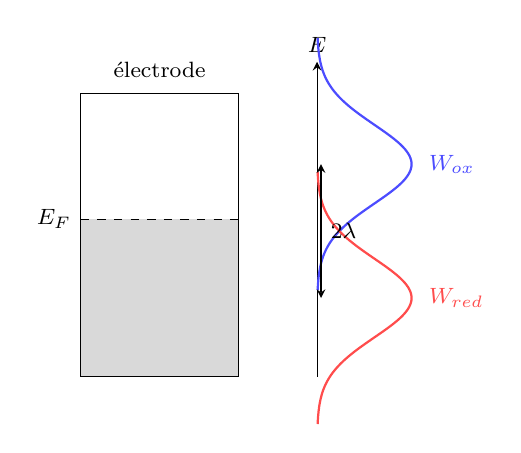
\begin{tikzpicture}[scale=1.0,>=stealth]
  % Electrode (gauche) : continuum rempli jusqu'au niveau de Fermi
  \fill[gray!30] (0,0) rectangle (2,2.0);
  \draw (0,0) rectangle (2,3.6);
  \node[align=center] at (1,3.9) {\footnotesize électrode};
  \draw[dashed] (0,2.0) -- (2,2.0);
  \node[left] at (0,2.0) {\footnotesize $E_F$};

  % Distributions redox (droite) : deux gaussiennes decalees de 2 lambda
  \draw[->] (3,0) -- (3,4.0) node[above] {\footnotesize $E$};
  % Ox (centree haut)
  \draw[thick,blue!70,domain=-1.6:1.6,smooth,samples=60,variable=\y]
    plot ({3 + 1.2*exp(-(\y)^2/0.5)},{2.7+\y});
  \node[blue!70,right] at (4.3,2.7) {\footnotesize $W_{ox}$};
  % Red (centree bas)
  \draw[thick,red!70,domain=-1.6:1.6,smooth,samples=60,variable=\y]
    plot ({3 + 1.2*exp(-(\y)^2/0.5)},{1.0+\y});
  \node[red!70,right] at (4.3,1.0) {\footnotesize $W_{red}$};

  % Ecart 2 lambda
  \draw[<->] (3.05,1.0) -- (3.05,2.7);
  \node[right] at (3.05,1.85) {\footnotesize $2\lambda$};
\end{tikzpicture}
\caption{Représentation à la Gerischer du transfert électronique à une
électrode : les états occupés de l'électrode (jusqu'au niveau de Fermi $E_F$)
échangent des électrons avec les distributions d'énergie des formes oxydée
($W_{ox}$) et réduite ($W_{red}$) du couple redox, élargies par la
réorganisation du solvant et séparées de $2\lambda$. Le courant est gouverné
par leur recouvrement.}
\label{fig:gerischer}
\end{figure}

\paragraph{Apports par rapport à Butler--Volmer.}
L'ensemble de ces formulations corrige plusieurs défauts de Butler--Volmer
\cite{henstridgeMarcusHushChidsey2012,
romanIdentifyingOptimalElectrocatalysts2017} :
\begin{itemize}
  \item le coefficient de transfert n'est plus constant : il varie avec la
        surtension, ce qui reproduit la courbure des tracés de Tafel ;
  \item le courant \emph{sature} à forte surtension (effet de la région
        inverse et de la densité finie d'états), au lieu de croître
        indéfiniment comme dans Butler--Volmer ;
  \item les paramètres ($\lambda$, densité d'états) ont un sens physique et se
        relient à la structure de l'espèce, du solvant et de l'électrode.
\end{itemize}

\paragraph{Hypothèses.}
Ces modèles reposent néanmoins sur des hypothèses qui restent fortes :
\begin{itemize}
  \item le transfert demeure \emph{mono-électronique} et élémentaire ;
  \item les surfaces d'énergie sont supposées paraboliques (réponse linéaire
        du milieu), avec une énergie de réorganisation $\lambda$ unique et
        constante ;
  \item le couplage électronique entre l'espèce et l'électrode est traité
        comme faible (régime non adiabatique).
\end{itemize}

\paragraph{Limites.}
Malgré une bien meilleure assise physique, ces formulations restent des
modèles de transfert mono-électronique entre une électrode et une espèce
redox. Elles ne décrivent pas en elles-mêmes les réactions à plusieurs
étapes ni les transferts couplés d'électrons et de protons. Pour la
réduction du \ce{CO2}, elles améliorent la description du transfert
élémentaire sans résoudre la question du mécanisme global.

% ------------------------------------------------------------
\subsection*{Application à notre cas : catalyseur moléculaire greffé}

Le catalyseur considéré dans ce travail est un complexe moléculaire greffé
sur les fibres de carbone. Ce contexte modifie la nature de la cinétique, et
aucun des modèles précédents ne s'y applique tel quel, mais la théorie de
Marcus en fournit le socle conceptuel.

\paragraph{Un cycle catalytique, pas un transfert unique.}
La réaction n'est pas un transfert électronique simple mais un cycle
catalytique : le complexe est d'abord réduit par le support carboné, puis
active et réduit le \ce{CO2} à travers une série d'intermédiaires, avant
d'être régénéré. Cette séquence relève de la catalyse moléculaire des
réactions électrochimiques \cite{saveantMolecularCatalysisElectrochemical2008, costentinCatalysisElectrochemicalReduction2013,
boutin<3MolecularCatalysis2020}, où le courant dépend du potentiel redox du
catalyseur, de la cinétique de chaque étape et de la densité de sites
greffés. Chacun des transferts électroniques internes au cycle peut, lui,
être décrit par une cinétique de type Marcus, ce qui fait de cette théorie le
cadre élémentaire pertinent à l'intérieur du mécanisme global.

\paragraph{Transferts couplés proton--électron.}
La réduction du \ce{CO2} en \ce{CO} met en jeu des transferts couplés
d'électrons et de protons (PCET). La force motrice et la barrière de chaque
étape dépendent alors conjointement du potentiel et du pH local
\cite{koperTheoryMultipleProton2013, gottleProtoncoupledElectronTransfer2017}.
Le PCET se formule comme une extension de la théorie de Marcus intégrant le
mouvement du proton et les états vibroniques associés
\cite{warburtonTheoreticalModelingElectrochemical2022}, ce qui relie
directement ce cadre à la description précédente.

\paragraph{Effet du greffage.}
Le greffage introduit enfin un transfert électronique entre le carbone et le
complexe, dont l'efficacité dépend du mode d'ancrage et du couplage
électronique. La cinétique pertinente se rapproche alors de celle des
catalyseurs moléculaires et des enzymes immobilisés étudiés en voltammétrie
\cite{fourmondModellingVoltammetryAdsorbed2017, le<3MultiscaleModelling2022,
zhangSingleMoleculeElectronTransfer2008}.

\paragraph{Où nous en sommes.}
À ce stade, la loi de Butler--Volmer est conservée comme première
approximation opérationnelle, faute d'une paramétrisation complète du cycle
catalytique de notre complexe. La trajectoire visée est néanmoins claire :
remplacer cette loi par une description fondée sur la théorie de Marcus pour
les transferts élémentaires, intégrée dans un cadre de catalyse moléculaire
décrivant le cycle complet et le couplage proton--électron. La construction de
ce modèle cinétique, et l'identification de ses paramètres pour notre
catalyseur, constituent une étape ultérieure de ce travail.


% ------------------------------------------------------------
\subsection*{Transferts couplés proton--électron et apport de la DFT}

La description précédente reste cinétique et macroscopique. Pour un
catalyseur moléculaire greffé réalisant la réduction du \ce{CO2}, deux
ingrédients supplémentaires doivent être pris en compte : le couplage entre
transfert d'électron et transfert de proton (PCET), et la nature des
intermédiaires réactionnels, accessibles par le calcul quantique.

\paragraph{Le couplage proton--électron.}
La réduction du \ce{CO2} en \ce{CO} requiert deux électrons et deux protons.
Le transfert de ces protons et électrons peut être \emph{concerté} (un proton
et un électron transférés en une seule étape) ou \emph{séquentiel} (transfert
d'électron puis de proton, ou l'inverse). Le chemin emprunté dépend du pH et
du potentiel, et détermine la dépendance en pH de l'activité et de la
sélectivité \cite{koperTheoryMultipleProton2013}. Le découplage des étapes
proton et électron introduit en particulier une dépendance forte au pH, avec
l'existence d'un pH optimal pour le turnover catalytique
\cite{koperTheoryMultipleProton2013}.

\paragraph{Formulation théorique du PCET.}
Le PCET se décrit comme une extension de la théorie de Marcus intégrant, en
plus de la coordonnée de réorganisation, le mouvement quantique du proton et
les états vibroniques associés \cite{warburtonTheoreticalModelingElectrochemical2022}.
La grandeur centrale reste l'énergie de réorganisation $\lambda$, mais elle
comporte désormais une contribution liée au proton, qui rend le PCET plus
coûteux que le transfert électronique seul. Cette extension a été validée
expérimentalement : pour un catalyseur greffé sur une électrode, l'énergie de
réorganisation du PCET interfacial peut être mesurée et se révèle nettement
supérieure à celle du transfert électronique pur
\cite{kessingerReorganizationEnergiesInterfacial2022}. Des cadres
mécanistiques récents relient cette description au caractère interfacial du
transfert, en distinguant le PCET vers une espèce en solution de celui vers
un site greffé \cite{lewisMolecularLevelMechanisticFramework}.

\paragraph{Apport des calculs de structure électronique (DFT).}
Les paramètres gouvernant ces étapes : potentiels redox des intermédiaires,
$\mathrm{p}K_a$, énergies d'activation, structure des adduits, ne sont pas
directement accessibles à une loi cinétique macroscopique. La théorie de la
fonctionnelle de la densité (DFT) permet de les calculer à l'échelle
moléculaire \cite{al-mahayniExperimentalMethodsChemical2021}. Pour la
réduction du \ce{CO2} sur des complexes moléculaires, ces calculs identifient
les intermédiaires (adduit carboxylate, espèces protonées), évaluent les
barrières des différentes étapes et prédisent la compétition entre chemins
concerté et séquentiel en fonction du pH
\cite{gottleProtoncoupledElectronTransfer2017}. Ce type d'analyse a été mené
en particulier sur des porphyrines de cobalt, proches de la famille de
catalyseurs visée dans ce travail \cite{gottleProtoncoupledElectronTransfer2017},
et plus largement sur les barrières de réaction du \ce{CO2RR}
\cite{TheoreticalUnderstandingElectrochemical2017}.

\paragraph{Articulation avec notre modèle.}
Ces approches micro\-scopiques (PCET, DFT) ne se substituent pas au modèle de
transport homogénéisé : elles en fournissent les \emph{paramètres cinétiques}
à l'échelle du site catalytique. Dans une démarche multi-échelle, les
constantes de vitesse calculées pour chaque étape élémentaire alimenteraient
le terme source réactionnel du modèle macroscopique, en remplacement de la
loi de Butler--Volmer globale. Cette articulation, calcul moléculaire des
étapes, puis intégration dans le modèle d'électrode, constitue la voie
envisagée pour une description cinétique fidèle de notre système.

% ------------------------------------------------------------
\subsection*{Modèles micro-cinétiques}

Les modèles précédents fournissent une loi globale reliant le courant à la
surtension. Une description plus fine consiste à ne pas résumer le cycle
catalytique en une loi unique, mais à écrire explicitement chaque étape
élémentaire — adsorption, transferts d'électrons et de protons, désorption —
avec sa propre constante de vitesse, puis à résoudre le système d'équations de
bilan sur les intermédiaires de surface. C'est le principe des modèles
micro-cinétiques (MKM).

Cette approche présente plusieurs avantages pour un catalyseur moléculaire
réalisant la réduction du \ce{CO2}. Elle décrit naturellement le caractère
multi-étapes et le changement d'étape limitante avec le potentiel, que les
lois globales ne reproduisent pas. Elle fait apparaître explicitement la
densité de sites et le couplage au pH local, à travers les étapes de transfert
de proton. Enfin, elle peut être alimentée par les paramètres calculés par
DFT (potentiels redox, $\mathrm{p}K_a$, barrières d'activation des étapes
élémentaires), ce qui en fait le point de jonction entre la description
moléculaire et le modèle d'électrode.

Une telle approche a été mise en \oe uvre pour la réduction du \ce{CO2} sur
catalyseur, en couplant un modèle micro-cinétique détaillé à un modèle de
transport de matière, précisément pour dépasser les limites de la loi de
Butler--Volmer \cite{adesinaButlerVolmerEquationCO22024}. Le prix à payer est
une complexité et un nombre de paramètres accrus : chaque étape élémentaire
introduit ses propres constantes, dont l'identification — par le calcul ou par
l'expérience — constitue la principale difficulté. Dans le cadre de ce
travail, le modèle micro-cinétique représente l'objectif à terme pour la
description de la cinétique interfaciale, une fois le cycle catalytique de
notre complexe suffisamment caractérisé.

% ------------------------------------------------------------
\subsection*{Comparaison des modèles cinétiques}

\begin{table}[htbp]
\centering
\renewcommand{\arraystretch}{1.3}
\begin{tabular}{p{2.7cm}p{3.2cm}p{3.2cm}p{3.6cm}}
\hline
 & \textbf{Butler--Volmer} & \textbf{Marcus / MHC} & \textbf{Catalyse moléculaire (PCET, DFT, MKM)} \\
\hline
Origine de la barrière & empirique (dans $j_0$, $\alpha$)
 & physique ($\lambda$, $\Delta G$, densité d'états)
 & étapes élémentaires calculées (DFT) \\
Coefficient de transfert & constant
 & variable avec $\eta$
 & non pertinent (mécanisme explicite) \\
Comportement à forte $\eta$ & croissance exponentielle
 & saturation (région inverse, densité d'états)
 & limité par le \emph{turnover} et la densité de sites \\
Nombre d'électrons & un (étape unique)
 & un (étape unique)
 & plusieurs, couplés aux protons (PCET) \\
Dépendance au pH & absente
 & absente
 & explicite (transferts de proton) \\
Électrode visée & métal massif
 & métal / semi-conducteur (Gerischer)
 & catalyseur moléculaire greffé \\
Niveau de description & loi globale
 & loi globale, transfert élémentaire
 & cycle catalytique résolu (MKM) \\
Paramètres requis & $j_0$, $\alpha$
 & $\lambda$, densité d'états
 & constantes de chaque étape (DFT / exp.) \\
Adapté à notre cas & non (approximation)
 & partiellement (transfert élémentaire)
 & oui (cadre cible) \\
\hline
\end{tabular}
\caption{Comparaison des modèles cinétiques au regard de la réduction du
\ce{CO2} sur catalyseur moléculaire greffé, du plus empirique (Butler--Volmer)
au plus détaillé (catalyse moléculaire avec PCET, paramétrée par DFT et
résolue par un modèle micro-cinétique). Butler--Volmer est retenu comme
première approximation ; la description cible relève de la dernière colonne.}
\label{tab:comparaison_cinetique}
\end{table}

% ------------------------------------------------------------
\paragraph{Lien avec le modèle de transport.}
Quel que soit le modèle cinétique retenu, son rôle dans la modélisation
développée ici est identique : fournir la relation $j(\eta, C_i)$ entre la
densité de courant interfaciale, la surtension locale et les concentrations,
qui ferme le terme source du système homogénéisé. C'est en effet cette
densité de courant qui détermine la vitesse de réaction interfaciale
$R_i = -\frac{\nu_i}{n_e F} j$, et donc le terme source volumique
$a_v^{\mathrm{cat}} R_i$ apparaissant dans l'équation de conservation
homogénéisée, ainsi que le terme $a_v^{\mathrm{cat}} j$ de la loi d'Ohm. Le
choix du modèle cinétique n'affecte pas la structure du modèle de transport :
il en fixe uniquement la fermeture interfaciale. Dans ce travail, cette
fermeture est assurée par la loi de Butler--Volmer, dont la linéarisation à
surtension constante fournit la cinétique du premier ordre
$j = k(\eta)\,C_i$ utilisée pour l'analyse par le module de Thiele. Le
remplacement de Butler--Volmer par une description de type Marcus ou par un
modèle de catalyse moléculaire reviendrait à modifier l'expression de
$j(\eta, C_i)$, sans changer l'architecture du modèle homogénéisé.

\paragraph{Régime de couplage transport--cinétique.}
La loi cinétique ne fixe pas seulement la fermeture interfaciale : elle
détermine aussi le régime de fonctionnement de l'électrode, à travers la
compétition entre la vitesse de réaction et celle du transport. Cette
compétition est mesurée par le module de Thiele $\phi$, dont la constante de
réaction $k(\eta)$ provient directement du modèle cinétique retenu. Lorsque la
cinétique est lente devant la diffusion ($\phi \ll 1$), la réaction est
limitante et la concentration reste uniforme dans l'épaisseur de l'électrode :
le courant est alors directement gouverné par la loi cinétique, et le choix de
celle-ci est déterminant. À l'inverse, lorsque la cinétique est rapide
($\phi \gg 1$), le transport devient limitant, la réaction se concentre près
de l'interface avec le bulk, et le détail de la loi cinétique influe moins sur
le comportement global. Le modèle cinétique et le modèle de transport sont
donc indissociables : c'est leur couplage, et non chacun pris isolément, qui
fixe les performances de l'électrode.